\documentclass[a4paper,11pt]{article}
\usepackage[a4paper, hmargin={1.5cm,1.5cm}, vmargin={1.5cm,1.5cm}]{geometry}
\usepackage{amsmath}
\usepackage{amsthm}
\usepackage{amsfonts}
\usepackage{color}
\usepackage[final]{graphicx}
\usepackage{subcaption}
\usepackage{wrapfig}
\newtheorem{remark}{Remark}[]
\newtheorem{prop}{Proposition}
\usepackage{amssymb}
\usepackage{enumitem}
\usepackage{tikz}
\usepackage{smartdiagram}
\usepackage{hyperref}

\newcommand{\R}{\mathbb{R}}
\newcommand{\C}{\mathbb{C}}
\newcommand{\N}{\mathbb{N}}
\newcommand{\Q}{\mathbb{Q}}
\newcommand{\W}{\mathbb{W}}
\newcommand{\Vspace}{\mathbb{V}}
\newcommand{\Hspace}{\mathbb{H}}
\newcommand{\Lspace}{\mathbb{L}}
\newcommand{\Lagr}{\mathcal{L}}


% Title Page
\title{Assignment 2 Applied Computational Science\\A Resume}
\author{Alifian Mahardhika Maulana}


\begin{document}
\maketitle
\section{About Simulation}
Simulation is an activity whether it's using computer or another experimental equipment to imitate phenomenon, real-world problem, machining process, material analysis, determining physical constant, etc. So that before doing something, we somehow know the risk and we can prepare before somethings bad happen. In computer simulation, we also can reproduce, understand, and predict.
\subsection{The Third Method}
In simulation, we should familiar with the third method about simulation, it is:
\begin{center}
	\smartdiagram[circular diagram:clockwise]{Theory,
		Experiment, Computational Science}
\end{center}
\begin{enumerate}[label=(\alph*)]
	\item Theory : Before we do a computational experiment, first we have to know the theory and if needed we have to derive the simplest solution to our problem so that our simulation run very fast.
	\item Experiment : With experiment, we confirm about the theory we use to derive the solution for the problem we face in the real-world.
	\item Computational Science : Computational science covered about high level theoretical calculation, including High Performance Computing (known as HPC) Computer to simulating and calculating a complex system of things like atom.
\end{enumerate}

\section{Super Computer}
K computer is one of the highest caliber of supercomputers in Japan. It is being used in a broad range of fields including drug discovery, earthquake/tsunami research, weather forecasting, space science, manufacturing and material development. It has 82944 nodes with each node has 16GB of memory and ability to compute 128 GigaFlop process. This K computer located in Kobe, Japan and can be accessed for scientists and researchers around the world to help them running a computational experiment.

\section{Molecular Simulation}
Molecular simulation help scientist or researcher to calculate and understand about molecular science in the field of Metal, liquid, chemical, biological molecule. A few example of molecular simulation are: Density Functional Theory, Molecular Dynamics Simulation, Monte Carlo Simulation. Computational Science, molecular simulation, basically use the law of physics to derive algorithm to do the programming for simulation, a few of the physical law are:
\begin{enumerate}[label=(\alph*)]
	\item Newton's equation of motion $\textbf{F}=m\textbf{a}$
	\item Schrodinger Equation $H\Psi = E\Psi$
	\item Thermodynamics, statistical mechanics
	\item Electromagnetic
\end{enumerate}
in this section we also learn about Lennard-Jones Potential System:
\begin{equation*}
U(r) = 4\bigg( \frac{1}{r^{12}} - \frac{1}{r^6}\bigg) \rightarrow f_x(r) = \frac{48x}{r^2}\bigg( \frac{1}{r^{12}} - \frac{1}{2} \cdot \frac{1}{r^6} \bigg)
\end{equation*}
which take most of the time when doing Molecular Dynamic (MD) Simulation almost 80\% from total computation time is needed in the calculation of the force acting on every particle. That's why before doing the simulation we have to know which one is the best algorithm to use, so that the calculation going faster.

\section{Simulation for Bio Material}
Human body are complex, it consist of 71\% Protein, 12\% Lipids, 7\% Nucleus Acid (DNA), 5\% Sugar, and 5\% for other than that. This is why simulation for bio material is important, to understand behaviour of the biological material inside human body, for advancing medical technology to save humanity. A few list of complex protein covered by bio material simulation are: Hemoglobin, Mioglobin, Lodopsin, Myosin, Keratin, and Fiber.
\subsection{Simulation of Protein Complex}
With the help of Molecular Dynamics Software, we can do a simulation for Bio Material. There is also an open source (free to download) data bank of protein at \url{http://pdb101.rcsb.org/}. One of the popular software for molecular dynamics simulation is Visual Molecular Dynamics (VMD), with the software we can calculate and analyze properties of the molecule, binding free energy, mean force, free energy profile, and also cavity density profile.
\begin{figure}[h!]
	\centering
	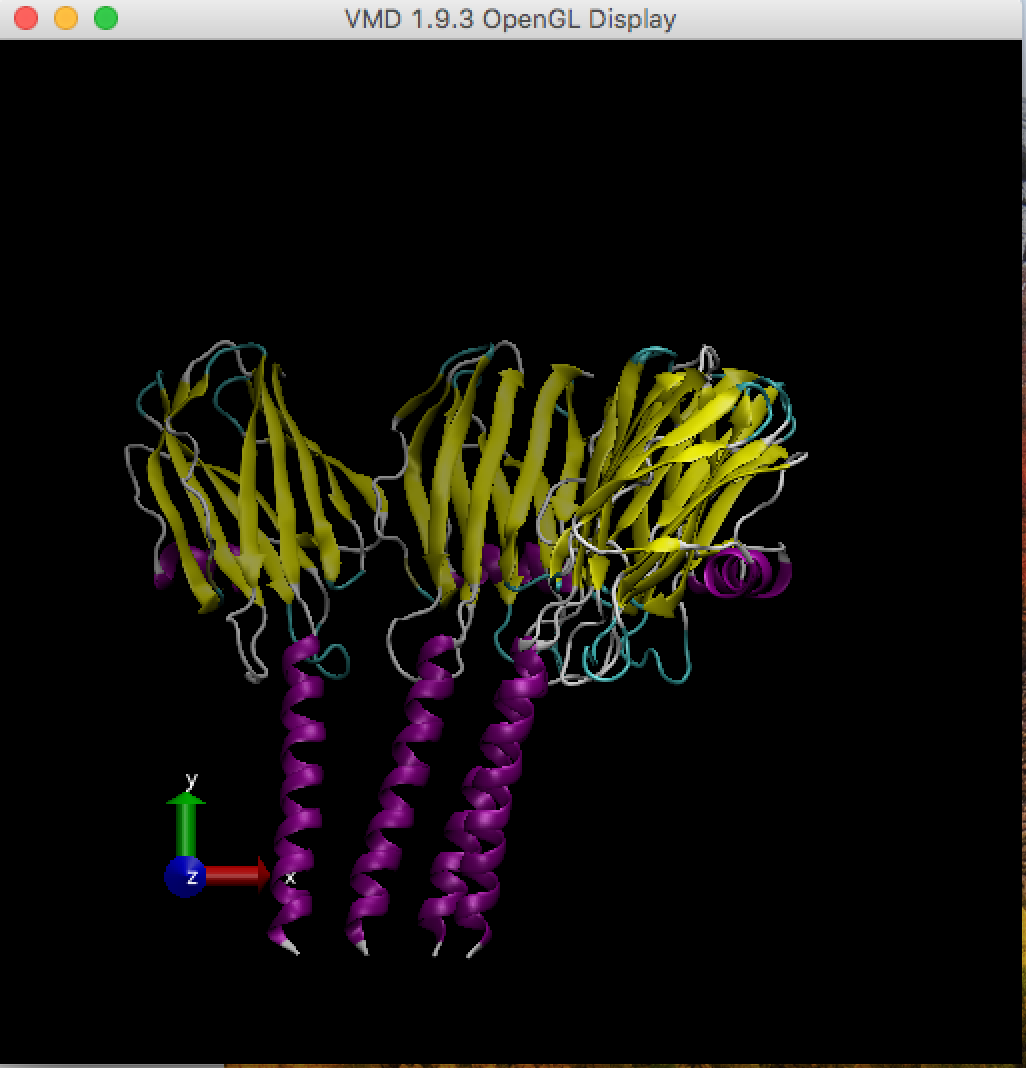
\includegraphics[width=0.37\linewidth]{picture/lipidfrac}
	\caption{An example of Crystal structure of FraC with lipids simulation using VMD}
	\label{fig:example1}
\end{figure}
\end{document}